\documentclass[12pt]{article}

% Packages
%%%%%%%%%%%
\usepackage{natbib}
\usepackage[francais]{babel}
\usepackage[T1]{fontenc}
\usepackage{url}
\usepackage[utf8x]{inputenc}
\usepackage{amsmath}
\usepackage{graphicx}
\graphicspath{{images/}}
\usepackage{parskip}
\usepackage{fancyhdr}
\usepackage{vmargin}
\usepackage[colorinlistoftodos]{todonotes}
\usepackage{titlesec}
\usepackage{wrapfig}
\usepackage[refpage]{nomencl}
\usepackage{lmodern}
\usepackage{pict2e}
%\usepackage{hyperref}

\newcommand{\benjamin}[1]{\textcolor{red}{#1}}
\newcommand{\pierre}[1]{\textcolor{green}{#1}}
\newcommand{\moi}[1]{\textcolor{blue}{#1}}

% Macros
%%%%%%%%%
\newcommand\licence{Licence 3 Informatique parcours Info / Miage / Math  Info}
\newcommand\univ{Faculté des sciences et technologies - Université de Lille}
\newcommand{\HRule}{\rule{\linewidth}{0.5mm}}
\newcommand\matiere{\textbf{Label Recherche} a sein de l'équipe \textit{FOX}}
\renewcommand{\footrulewidth}{0.6pt}

\title{Reconnaissance d'émotions par réseaux de neurones à Spikes}
\author{Alexandre Hulsken}

\setlength{\unitlength}{1cm}


% Displaying
%%%%%%%%%%%%%
\setmarginsrb{2.5 cm}{2.5 cm}{2.5 cm}{2.5 cm}{1 cm}{1.5 cm}{1 cm}{1.5 cm}
\titlelabel{\thetitle. \quad}
\titleformat{\section}{\LARGE\scshape\raggedright\bfseries}{}{1.5em}{}[\titlerule\vspace{0.3em}]
\titlelabel{\thetitle. \quad}

\makeatletter
\let\thetitle\@title
\let\theauthor\@author
\makeatother


% Params
%%%%%%%%%

\pagestyle{fancy}
\fancyhf{}
\lhead{\footnotesize \licence – \univ}
\rfoot{\thepage}
\lfoot{\footnotesize \theauthor}
\makenomenclature

%%%%%%%%%%%%%%%%%%%%%%%%%%%%%%%%%
%%  BEGINNING OF THE DOCUMENT  %%
%%%%%%%%%%%%%%%%%%%%%%%%%%%%%%%%%


\begin{document}

%%%%%%%%%%%%%%%%%%
%%  FIRST PAGE  %%
%%%%%%%%%%%%%%%%%%

\begin{titlepage}
\center

\textsc{\LARGE \univ}\\[1.5cm]
\textsc{\licence}\\[0.5cm]
\textsc{\large \matiere}\\[0.5cm]

\HRule \\[0.4cm]
{ \huge \bfseries \thetitle}\\[0.4cm]
\HRule \\[1.5cm]

\begin{minipage}{0.4\textwidth}
\begin{flushleft} \large
\emph{Étudiant :}\\
Alexandre \textsc{Hulsken}
\end{flushleft}
\end{minipage}
~
\begin{minipage}{0.4\textwidth}
\begin{flushright} \large
\emph{Encadrants :} \\
Pierre \textsc{Tirilly}\\
Benjamin \textsc{Allaert}
\end{flushright}
\end{minipage}\\[1.7cm]

{\large Janvier-Avril 2018}\\[1.5cm]


\includegraphics[scale=0.5]{logoCRIStAL.png} \hspace{0.5cm}

\includegraphics[scale=0.15]{logoFOX.png}\\[1cm]

\includegraphics[scale=0.3]{logo.png}

\pagebreak

\end{titlepage}


%%%%%%%%%%%%%%%%%%%%
%%  CONTENT PAGE  %%
%%%%%%%%%%%%%%%%%%%%
\setcounter{page}{0}
\renewcommand{\contentsname}{Sommaire}
\tableofcontents
\thispagestyle{empty}

\pagebreak

%%%%%%%%%%%%%
%%  INTRO  %%
%%%%%%%%%%%%%
\section{Introduction}

Dans le cadre de ma dernière année de Licence Informatique à l'université des Sciences et Technologies de Lille, j'ai pu suivre cette option qui est le Label Recherche. Le présent rapport qui suit retracera donc le travail qu'il m'a été donné de fournir.

\subsection{Environnement}

Dans le monde, le nombre d'informations disponibles est immense. Et même si l'on ne se restreint seulement aux informations visuelles, il reste une abondante quantité de ces dites informations. Ce sont des données difficiles à analyser à cause de cette richesse (la palette de couleurs, les différentes textures, les mouvements possibles, les positions dans l'espace, la variabilité d'apparence de l’information, etc...), ce qui introduit ainsi diverses problématiques lorsque l'on souhaite les analyser.

C'est pourquoi l'équipe de recherche FOX (Fouille et indexation de dOcuments compleXes et multimédia) s'est positionné sur le problème des difficultés d'analyses de ces informations multiples. Ils travaillent ainsi sur de nouvelles techniques dans ce large domaine tel que l'étude de descripteurs de mouvement pour détecter et suivre les objets mobiles. Ils considèrent donc les quatre grands domaines de validations : le regard, l’événement l'émotion et la reconnaissance de personne réalisé à deux niveau d'échelles : l'individu et les flux.

Mon projet porte donc sur un domaine bien précis de ces différentes thématiques qui est la reconnaissance émotionnel d'individu.

\subsection{Contexte}

L'expression faciale est l'un des traits les plus important dans le domaine de la reconnaissance d'expression faciale\cite{darwin}. Mais de nos jours automatiser ce travail et ne plus le laisser exclusivement aux êtres vivants est un réel défi. En effet, avec le déploiement et les avancées des agents conversationnels et de la robotique qu'il nous a été donné d'observer ces dernières années, leur apprendre à pouvoir faire cette même extraction d'informations pourrait permettre de pousser encore beaucoup plus loin les technologies déjà créées. %C'est pourquoi ces dernière années ont aussi été très fructueuse dans le domaine de la reconnaissance d'émotions qu'il a pu devenir un sujet de recherche de plus en plus répandu.

Ce travail de reconnaissance d'émotions consiste donc à inférer l'état émotionnel d'une personne (joie, peur, colère, etc...) à partir de signaux acquis par différents capteurs (visuels, audios, données physiologiques...). Dans ce projet nous nous intéressons à l'analyse des expressions faciales sur des images statiques.

Le passage du signal d'entrée à l'émotion est généralement réalisé à l'aide d'un algorithme d'apprentissage automatique. Dans ce projet nous nous intéressons à la détection des expressions faciales dans les images à l'aide de modèles d'apprentissage de type réseaux de neurones impulsionnels.

\subsection{Problématique}

Ces réseaux de neurones, plus proches du modèle biologique que les modèles classiques de type perceptron, sont prometteurs, mais leur fonctionnement est encore mal compris. Leur application à des problématiques réelles, comme la reconnaissance d'émotions, demande donc un travail important d'exploration des architectures de réseaux et de leurs paramètres, sur des sous-problèmes de difficulté croissante.

\subsection{Objectifs}

L'objectif est d'identifier un sous-problème et d'effectuer des expérimentations permettant d'évaluer les modèles de réseaux de neurones impulsionnels déjà utilisés dans l'équipe sur chacun de ce sous-problème. Le travail réalisé consiste donc à :

\begin{itemize}
\item identifier un sous-problème à traiter;
\item préparer les données correspondant à ce sous-problème;
\item effectuer les expérimentations;
\item évaluer et analyser les résultats obtenus.
\end{itemize}

\subsection{Plan}

Dans la suite de ce rapport vous pourrez trouver un état de l'art dans la section suivante. La Section 3, quand à elle, parlera du travail de prétraitement des images qui sera suivi par la phase expérimentale dans la section 4. Enfin, je conclurai dans la section 5.

\pagebreak

%%%%%%%%%%%%%%%%%%%%%
%%  Etat de l'art  %%
%%%%%%%%%%%%%%%%%%%%%
\section{État de l'art}

\subsection{Processus d'analyse des expressions faciales}

Ce sujet de recherche ayant eu un engouement particulier ces dernières années, il a été possible de voir l'émergence de différentes familles dans l'approche de l'analyse des expressions faciales.

\subsubsection{Les méthodes traditionnelles}

Le mécanisme de reconnaissance d'expressions faciales peut se décomposer en trois grandes différentes étapes\cite{LiJain} comme l'on peut le voire ci-dessous:

\begin{picture}(8,4)
	% Les étapes
    \put(0,3.3){\underline{\textbf{Étape 1 :}}}
    \put(0,1.8){\underline{\textbf{Étape 2 :}}}
    \put(0,0.3){\underline{\textbf{Étape 3 :}}}
    
	% Les boîtes
    \put(6,3){\framebox(4, 0.8)[c]{Acquisition faciale}}
    \put(4,1.5){\framebox(8, 0.8)[c]{Extraction et représentation de la donnée}}
	\put(6.5,0){\framebox(3, 0.8)[c]{Classification}}
    
	% Les flèches entre les boîtes
    \put(8,3){\vector(0,-1){0.7}}
    \put(8,1.5){\vector(0,-1){0.7}}
\end{picture}

%\begin{itemize}
%\item L'acquisition faciale;
%\item L'extraction et la représentation de la donnée;
%\item La classification.
%\end{itemize}

%\benjamin{n'hésites pas à illustrer avec une image illustrant les différentes étapes.}

% \paragraph{paragraph about $\Rightarrow$ facial acquisition $\rightarrow$ face detection / landmarks / headpose estimation}
L'acquisition faciale, ou plus communément prétraitement de l'image, consiste à devoir trouver où se situe l'information que l'on va traiter dans l'ensemble de l'image et ensuite de la préparer pour la suite. La méthode la plus largement utilisé est d'extraire les points du visage. Pour les détecter, il existe différentes méthodes tel que les algorithmes de régression\cite{art1}. Ces différents points servent alors à savoir où se trouve certaines informations (tel que le nez, un coin de la bouche, les yeux, etc...) en fonctions de leurs coordonnées dans l'images et permettent donc par la suite d'avoir une estimation de la position de la tête du sujet dans l'espace et d'en extraire le visage que l'on souhaite traiter du reste de son environnement.

Dans les travaux qui ont été effectué sur l'extraction et la représentation des données, deux principaux modèles sont apparus. Le premier basé sur la géométrie fonctionne sur le fait d'extraire la forme ainsi que la localisation de partie du visage tel que la bouche, les yeux, le nez, etc... Ce modèle étant souvent couplé avec un FACS (Facial Action Coding System), qui permet de diviser une émotion en différents mouvements types ainsi que de leur intensité sur des zones spécifiques du visage tel que le plissement sur le haut du nez plus au moins fort, l'ouverture de la bouche ou un haussement de sourcil. Mais grâce aux travaux de Shan, Gong et McOwan\cite{ShanGongMc}, l'importance de la qualité de l'image à pu être mise en évidence sur les résultats ce modèle alors qu'elle importe peu sur les méthodes d'extraction basé sur l'apparence (il faut noté que les travaux se basant sur la géométrie se base également sur l'apparence pour reconnaître les unités d'actions utiles pour le FACS). Cette dernière extrait l'information de l'émotion sur l'ensemble du visage après application de certains filtres. Mais dans chacun des cas, la représentation du la donnée extraite se fait par des vecteurs représentant chaque pixels de l'image que l'on souhaite traiter.

Une fois ce travail effectué, il ne reste plus que la classification. Selon Liu, Han, Meng et Tong\cite{LiuHanMengTong}, la phase de classification possède trois phases dans son apprentissage. La première étant l'acquisition de modèles suivi par une sélection de ces modèles qui a pour but de maximiser la différence entre les différences des descripteurs inter-classes et de minimiser les différences intra-classes. Suite à cela on passe enfin à la construction du ou des classifieurs qui permettront de classer leurs entrées en une seule et unique sortie correspondant à une émotion.

\subsubsection{Les méthodes de deep learning}

L'évolution dans le domaine de l'Intelligence Artificielle, et plus précisément dans les réseaux de neurones, a permis de faire d'énormes avancées dans le domaine de la vision artificielle. En effet, les réseaux de neurones convolutifs, de type MLP (MultiLayer Perceptron) grâce aux travaux de Lecun\cite{lecun}, utilisé dans la phase d'extraction de modèle a déjà permis de simplifier l'ensemble du processus de reconnaissance. Ils ont notamment simplifier le traitement des données puisque supportant des images brutes, il ne devient plus nécessaire de coder à la main l'ensemble de données sous certains formats, et il est donc possible d'entrer des images sous forme d'un vecteur de pixel. Ils ont également simplifier l'ensemble du traitement en fusionnant les étapes d'extraction et de classification (étapes 2 et 3) en une seule puisqu'ils sont capables de traiter les données et de retourner des entiers à leur sortie, ce qui correspond au label d'une classe (et dans notre cas à une émotion) tout ça en ayant de très bon résultats de réussite.%\benjamin{c'est tout sur ce sujet ?, qu'est ce que cela implique pour les données en entrée ? comment sont calculés les expressions au sein d'un CNN ? existe-t-il des architectures mieux adaptées ?}

L'expérimentation de ces architectures d’apprentissage automatique se fait en séparant l'ensemble des données en deux sous-ensembles différents. L'un de ces derniers est donc utilisé pour l'apprentissage du réseau et le second pour son test. Ce cloisonnement a pour but de ne pas fausser les résultats de la phase expérimentale de l'architecture en ne faisant pas de test sur des images déjà apprises par le réseau.

%\benjamin{n'hésites pas à illustrer avec une image, en lien avec les expressions faciales si possible}

\subsection{Les Réseaux de neurones impulsionnels}

Les réseaux de neurones impulsionnels ont une représentation similaire aux convolutifs. Ils sont constitués de neurones ayant plusieurs synapses d'entrés et un de sortie, et sont disposés également sous forme de couches. Mais malgré cela, ils possèdent un mode de très fonctionnement différents.

\subsubsection{Le STDP neurone}

\begin{wrapfigure}{r}{70mm}
	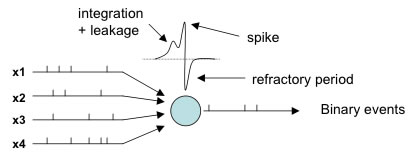
\includegraphics[scale=0.5]{data/neurone.jpg}
    \caption{Schéma d'un neurone impulsionnel}
    \label{neurone}
\end{wrapfigure}

Le neurone impulsionnel, à la différence de neurone convolutif, fonctionne grâce à une  simulation d'impulsions électrique et la notion importante dans leurs utilisations est la notion de temps entre ces dites impulsions. Ils sont caractérisés par un ensemble de synapses (post et pré synaptiques) ainsi qu'un potentiel électrique, d'une fonction de déperdition et d'un seuil d'activation\ref{neurone}. Leur fonctionnement étant que pour chaque impulsion pré-synaptique, la charge électrique du neurone augmente, et lors du temps où il n'est pas sollicité, cette charge diminue en fonction de leur fonction de déperdition. Ensuite lorsque cette charge dépassera le seuil du neurone, elle sera réinitialisé et le neurone enverra une impulsion post-synaptique.

Il fonctionne également grâce à des poids sur ses synapses d'entrées, mais ici leur modification change de manière différente. Le principe sous-jacent est le même que celui du modèle biologique et se nomme la plasticité en fonction du temps d’occurrence des impulsions\cite{art5} (ou en anglais, Spike-timing-dependent plasticity, STDP). Il s'agit d'une règle d’apprentissage qui fonctionne en modifiant en regardant quand un synapse va emmètre une impulsion de sortie. Lorsque ce sera le cas, le principe sera d'augmenter le poids des synapses d'entrés ayant été activé avant l’émission de la sortie et va diminuer le poids de ceux qui seront activer après cette émission. Cette augmentation (ou diminution) du poids du synapse sera plus ou moins importante en fonction du temps entre l'impulsion d'entrée et celle de sortie (plus elles seront proches, plus la modification sera importante). Ce principe d'apprentissage du neurone est importante puisqu'elle implique une autre grande différence avec les modèles de réseaux de neurones traditionnels puisqu'il nous n'avons donc plus besoin de rétro-propagation pour l'apprentissage.

\subsubsection{Une architecture particulière}

Les réseaux de neurones impulsionnels possèdent une architecture assez particulière, puisque dans la plus grande majeur partie des cas, ne sont disposés qu'en une seule et unique couche. Une autre particularité est qu'en plus des synapses d'entrées/sorties, il existe également une deuxième catégorie de synapses appelé LIF\cite{art4} (Leaky-Integrate-and-Fire) qui relie chaque neurone avec le reste des autres. Ils ont pour but d'empêcher l'apprentissage du même modèle par plusieurs neurones. Ils sont chacun activé lorsqu'un neurone envoie une impulsion post-synaptique et lance une face inhibitrice des autres neurones durant laquelle ils laisseront leur potentiel électrique redescendre jusqu'à être nul.

Cette architecture de réseaux de neurones à Spikes sont plus proche du modèle biologique que les modèles classiques de deep learning. C'est pourquoi nous travaillerons dans la suite avec ce modèle d'architecture pour mon projet de recherche.

%\benjamin{n'hésites pas à illustrer avec une image, en lien avec les expressions faciales si possible}

\pagebreak

%\benjamin{il est important de faire une petite conclusion dans cette section, pour dire pourquoi nous souhaitons faire du SNN. Et il faut une transition vers la section suivante.}

%%%%%%%%%%%%%%%%%%%%%%
%%  PRE-PROCESSING  %%
%%%%%%%%%%%%%%%%%%%%%%
\section{Le prétraitement des données}

La première partie de mon travail portait sur le prétraitement des images. La figure \ref{preprocessing} représente le processus que j'ai implémenté avec une image extraite de la base de donnée ADFES.

\begin{figure}
    \begin{picture}(10, 7)
        % Les images
        \put(0.1, 3.5){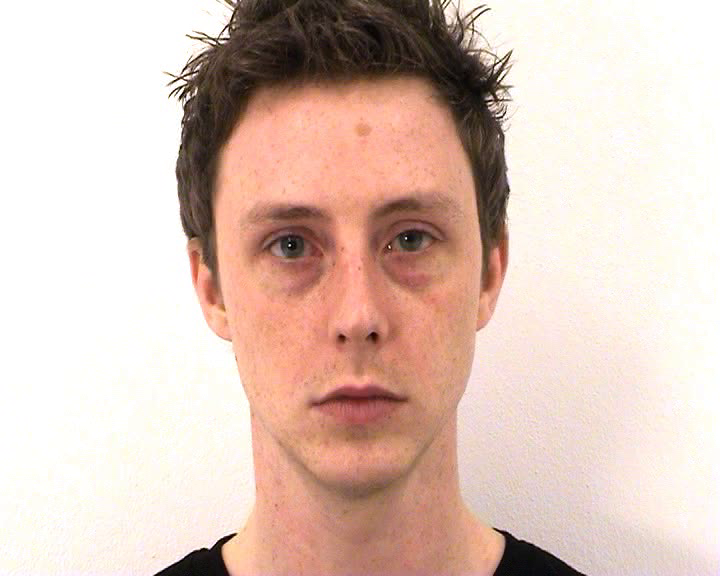
\includegraphics[scale=0.15]{prossessing_img/img_001.png}}
        \put(0.6, 0.7){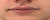
\includegraphics[scale=1.4]{prossessing_img/cropped.png}}
        \put(4.6, 0.7){
\includegraphics[scale=1.4]{prossessing_img/grayscale.png}}
        \put(8.6, 0.1){
\includegraphics[scale=1.4]{prossessing_img/dog_on.png}}
        \put(8.6, 1.3){
\includegraphics[scale=1.4]{prossessing_img/dog_off.png}}

        % box
        \put(0.2, 2.3){\shortstack{Processus de traitement}}
        \put(0, 0){\line(1, 0){11.6}}
        \put(0, 2.4){\line(1, 0){0.15}}
        \put(4.6, 2.4){\line(1, 0){7}}
        \put(0, 0){\line(0, 1){2.4}}
        \put(11.6, 0){\line(0, 1){2.4}}

        % Les flèches
        \put(2, 3.5){\vector(0, -1){1}}
        \put(3.05, 1.2){\vector(1, 0){1.5}}
        \put(7.05, 1.2){\vector(1, 0.4){1.5}}
        \put(7.05, 1.2){\vector(1, -0.4){1.5}}

        \put(11.05, 1.8){\vector(1, 0){1.5}}
        \put(11.05, 0.6){\vector(1, 0){1.5}}

        % textes
        \put(2.2, 2.9){\shortstack{image d'entrée}}
        \put(12.58, 1.7){\shortstack{DoG off}}
        \put(12.58, 0.5){\shortstack{DoG on}}
    \end{picture}

\caption{Schéma du processus de prétraitement mise en place}
\label{preprocessing}
\end{figure}


\subsection{La normalisation des données}

\begin{figure}
	\centering
  	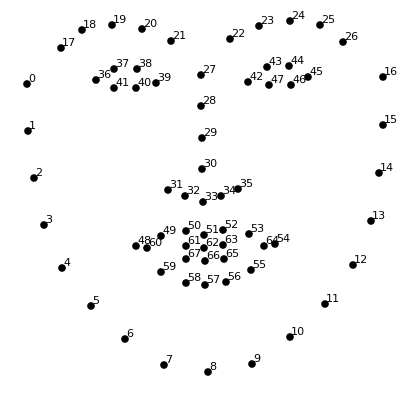
\includegraphics[scale=0.40]{landmarks.png}
  	\caption{Schéma représentant les points du visage}
  	\label{landmarks}
\end{figure}

Mon travail de prétraitement des données a ainsi commencé par extraire la partie importante du visage que je souhaitais utiliser. Pour cela j'ai donc utilisé les points du visage (un modèle à 68 points tel qu'ils sont représentés dans la figure \ref{landmarks}) afin de pouvoir découper cette image grâce à la bibliothèque OpenCv et ne garder uniquement la partie qui me servirai pour la suite. J'ai également dû redimensionner l'image résultante en une taille prédéfinie afin de normaliser l'ensemble des images ce qui permettait par la suite de travailler avec le réseau de neurones à spikes.

\subsection{L'extraction des contours}

J'ai ensuite dû transformer ces images couleurs en noirs et blancs. Ce qui m'a ensuite permis de pouvoir appliquer un algorithme d'extraction des contours (dernière étape du processus de prétraitement représenté dans la figure \ref{preprocessing}) fonctionnant sur un algorithme de différences de gaussiennes (DoG). Le principe fonctionne sur le fait que pour chaque pixel de coordonnées (x, y) on utilise un flou gaussien se modélisant sous la formule suivante :

\[
	G_\sigma(x, y) = \dfrac{1}{\sqrt[]{2\pi\sigma^2}}\exp(-\dfrac{x^2 + y^2}{2\sigma^2})
\]

Où $\sigma$ le paramètre du flou. Ensuite, il a fallu faire une soustraction pixel par pixel de deux flous paramétrées différemment (il est important que le paramètre $\sigma$ soit différent pour ces deux flous, sinon l'extraction échouera). Finalement, la différenciation on/off du résultat se fait en ne retenant uniquement les valeurs positives(on) ou négative(off).

\pagebreak

%%%%%%%%%%%
%%  EXP  %%
%%%%%%%%%%%
\section{L'expérimentation}

Il s'agissait maintenant, après avoir mis en place le processus de traitement de mes données, de tester l'architecture déjà utilisé dans l'équipe, pour cela nous allons voire quel à été ma démarche expérimentale.

\subsection{Les bases de données}

Pour l'expérimentation de l'architecture utilisé, nous avons utilisé la base de données CK+\cite{ck} (The Extended Cohn-Kanade database). Il s'agit d'une base très utilisé dans le domaine de la reconnaissance d'expressions faciales ce qui pourra nous aider dans la comparaison avec d'autres modèles déjà existant. Cette base étant constitué des 6 expressions basiques (la colère, le dégoût, la peur, la joie, la tristesse et la surprise) et d'une expression non basique (le mépris). Elle est ainsi divisée en 327 séquences d'images commençant par l'émotion neutre et allant jusqu'à l'apex, qui est le sommet de l'émotion, joué par 118 sujets.

J'ai également utilisé la base de données ADFES\cite{adfes} (The Amsterdam Dynamic Facial Expression Set) ayant la même structure mais proposant un plus grand panel d'émotions non basiques (avec l'embarras et la fierté en plus). Tout cela joué par 22 sujets (10 femmes et 12 hommes).

\begin{figure}
    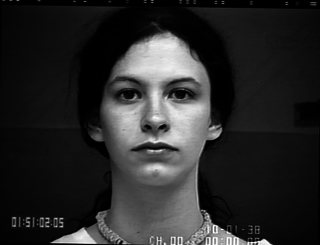
\includegraphics[height=3cm]{data/img_0012_ck.png}
    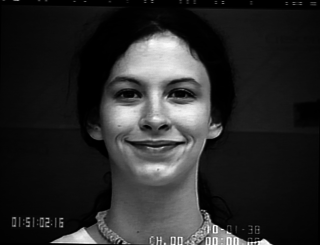
\includegraphics[height=3cm]{data/img_0122_ck.png}
    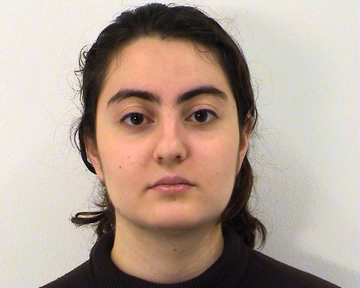
\includegraphics[height=3cm]{data/img_0012_adfes.png}
    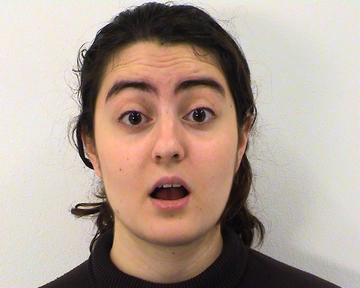
\includegraphics[height=3cm]{data/img_1502_adfes.png}
    \caption{A gauche se trouve deux images extraites de CK+ (représentant un visage neutre et souriant) et à droite deux autres extraites de ADFES (représentant l'émotion neutre et la surprise).}
    \label{datas}
\end{figure}

Ces deux bases, représenté dans la figure \ref{datas}, ont notamment des conditions d'acquisitions excellentes pour l'analyse puisque, comme étant faite en laboratoire, elles disposent des visages frontales dans une éclairage suffisant et homogène avec des expressions intenses et une bonne qualité de résolution. C'est pour cela que nous avons choisi d'effectuer les tests de l'architecture sur ces dites-bases.

\subsection{Le test de l'architecture du réseaux de neurones}

Sur l'architecture que je souhaitais utiliser nous avons donc l'ensemble du prétraitement précédent pour l'acquisition (étape 1). Ensuite, nous avons donc Le réseaux de neurone pour l'extraction de modèle (étape 2) et nous utilisons une SVM (Support Vector Machine) pour la classification (étape 3). 

\subsubsection{Test de la difficulté du problème}

Afin de tester la difficulté du problème que je mettais en place, et pour avoir une base de résultats afin de voire l'efficacité de l'utilisation d'un réseau de neurones impulsionnel, j'ai lancé une phase de test de l'architecture entrant les résultats du prétraitement directement dans la SVM (qui, comme le réseau de neurones, doit avoir une phase d'apprentissage) ce qui m'a permis d'obtenir les résultats que vous pourrez observer dans le tableau \ref{res} (un schéma de l'architecture du test se trouve sur la figure \ref{svm} en annexe). %\benjamin{attention, ici ce n'est pas les pourcentage obtenus en utilisant les pixels mais plutôt ceux obtenus avec les contours, ce qui sera plus logique par rapport à ce que tu cherches à évaluer avec les SNNs.}

\begin{table}
\begin{tabular}{|c|c|c|c|}
\hline Ensemble d’entraînement & ensemble de test & DoG & taux de reconnaissance \\
\hline training set & testing set & on & 100 \% \\
training set & testing set & off & 100 \% \\
testing set & training set & on & 99,4 \% \\
testing set & training set & off & 99,64 \% \\ \hline\hline
ADFES & CK+ & on & 74,2 \% \\
ADFES & CK+ & off & 74,7 \% \\
CK+ & ADFFES & on & 79,6 \%\\
CK+ & ADFFES & off & 81,4 \%\\ \hline
\end{tabular}
\caption{Tableau des premiers résultats expérimentaux}
\label{res}
\end{table}

Dans cette phase de test j'ai donc mis en place deux protocoles de test différents, le premier étant un training/testing set où j'ai créé un ensemble en fusionnant les deux bases. J'ai ensuite extrait un nombre nombre prédéfini d'image de cette ensemble pour les mettre dans l'ensemble de test, le reste servait donc à l'ensemble d’entraînement. Le second protocole étant de la cross-dataset validation où l'on prend tout simplement une base pour l'apprentissage et l'autre base pour le test.

\subsubsection{Le protocole expérimental}

Au vu des résultats précédents, On a pu déduire que le problème était assez simple (puisque l'ensemble des résultats sont élevés). Mais ils ont également pu soulever des problèmes se trouvant dans le premier protocole puisque les résultats sont beaucoup trop proches de la classification parfaite. Après analyse, il en est ressorti des problèmes dans la construction de ces ensembles de ce protocole, tel que le fait que les sujets pouvaient apparaître dans les deux ensembles, que plusieurs images était se ressemblaient au point d'être quasiment identiques et que certaine classe était en surpopulation. Il s'agit effectivement d'un problème falsifiant la fiabilité des tests puisque l'on testait l'architecture sur des images qu'il connaissait déjà.

Suite à ces premiers résultats j'ai fait le choix construire un protocole expérimental se basant sur la cross-dataset validation. J'ai donc fait un apprentissage du réseau de neurone sur une base. Suite à cela, il faut testé cette même base dans le réseau une fois qu'il était entraîné afin de pouvoir connaître le comportement qu'il a sur se qu'il connaît déjà afin de pouvoir utilisé se résultat comme base d'apprentissage pour la SVM. Finalement, il faudra testé l'architecture obtenu sur la deuxième base (vous pourrez trouver un schéma illustrant ce protocole se trouve en annexe sur la figure \ref{archi}).

\pagebreak

%%%%%%%%%%%
%%  CCL  %%
%%%%%%%%%%%
\section{Conclusion}

Dans le cadre de ce projet de recherche, j'ai travaillé sur la reconnaissance d'expression faciale d'un individu dans des images. Plus précisément, mes contributions se portaient sur deux parties différentes dans l'utilisation d'un réseau de neurones impulsionnels. D'une part, sur le processus de prétraitement des données en mettant en place un processus complet permettant d'extraire les contours d'une image sur la zone particulière de l'image qui nous intéresse. J'ai également pu travailler sur la mise en place d'un protocole d'expérimentation de ce dit réseau.

Nous pourrions donc envisager pour le future de ce projet d'augmenter la difficulté en plusieurs autres sous problèmes de la reconnaissance d'expression faciale en travaillant sur une autre zone du visage (comme les yeux ou le nez) ou sur plusieurs zone en même temps voir même sur le visage complet.

\pagebreak

%%%%%%%%%%%%%%%%%
%%  THANKS TO  %%
%%%%%%%%%%%%%%%%%
\section*{Remerciement}

Je tiens tout particulièrement à remercier mes encadrants, Benjamin Allaert et Pierre Tirilly, pour m'avoir pris sous leurs ailes lors de ce Label Recherche. Je tenais à les remercier également d'avoir répondu à toutes mes questions et de m'avoir fait confiance lors de ce temps passé ensemble.

Je remercie aussi toute l'équipe FOX et l'IRCICA pour m'avoir accueilli chez eux.

Merci aussi à toute l'équipe pédagogique sans qui cette option ne serait pas là et aucun étudiant de Licence 3 n'aurait pu découvrir le monde de la recherche aussi tôt.

Je voudrais finalement dire merci aux amis suivants cette même option. Ils m'ont écouté et également posé des questions sur ce que je faisais avec intérêt ce qui m'a permis de trouver des solutions par moi-même à des problèmes et avancer encore plus loin.

\thispagestyle{empty}
\pagebreak

%%%%%%%%%%%%%%
%%  ANNEXE  %%
%%%%%%%%%%%%%%
\appendix
\section*{ANNEXE A :}
\begin{figure}[h!]
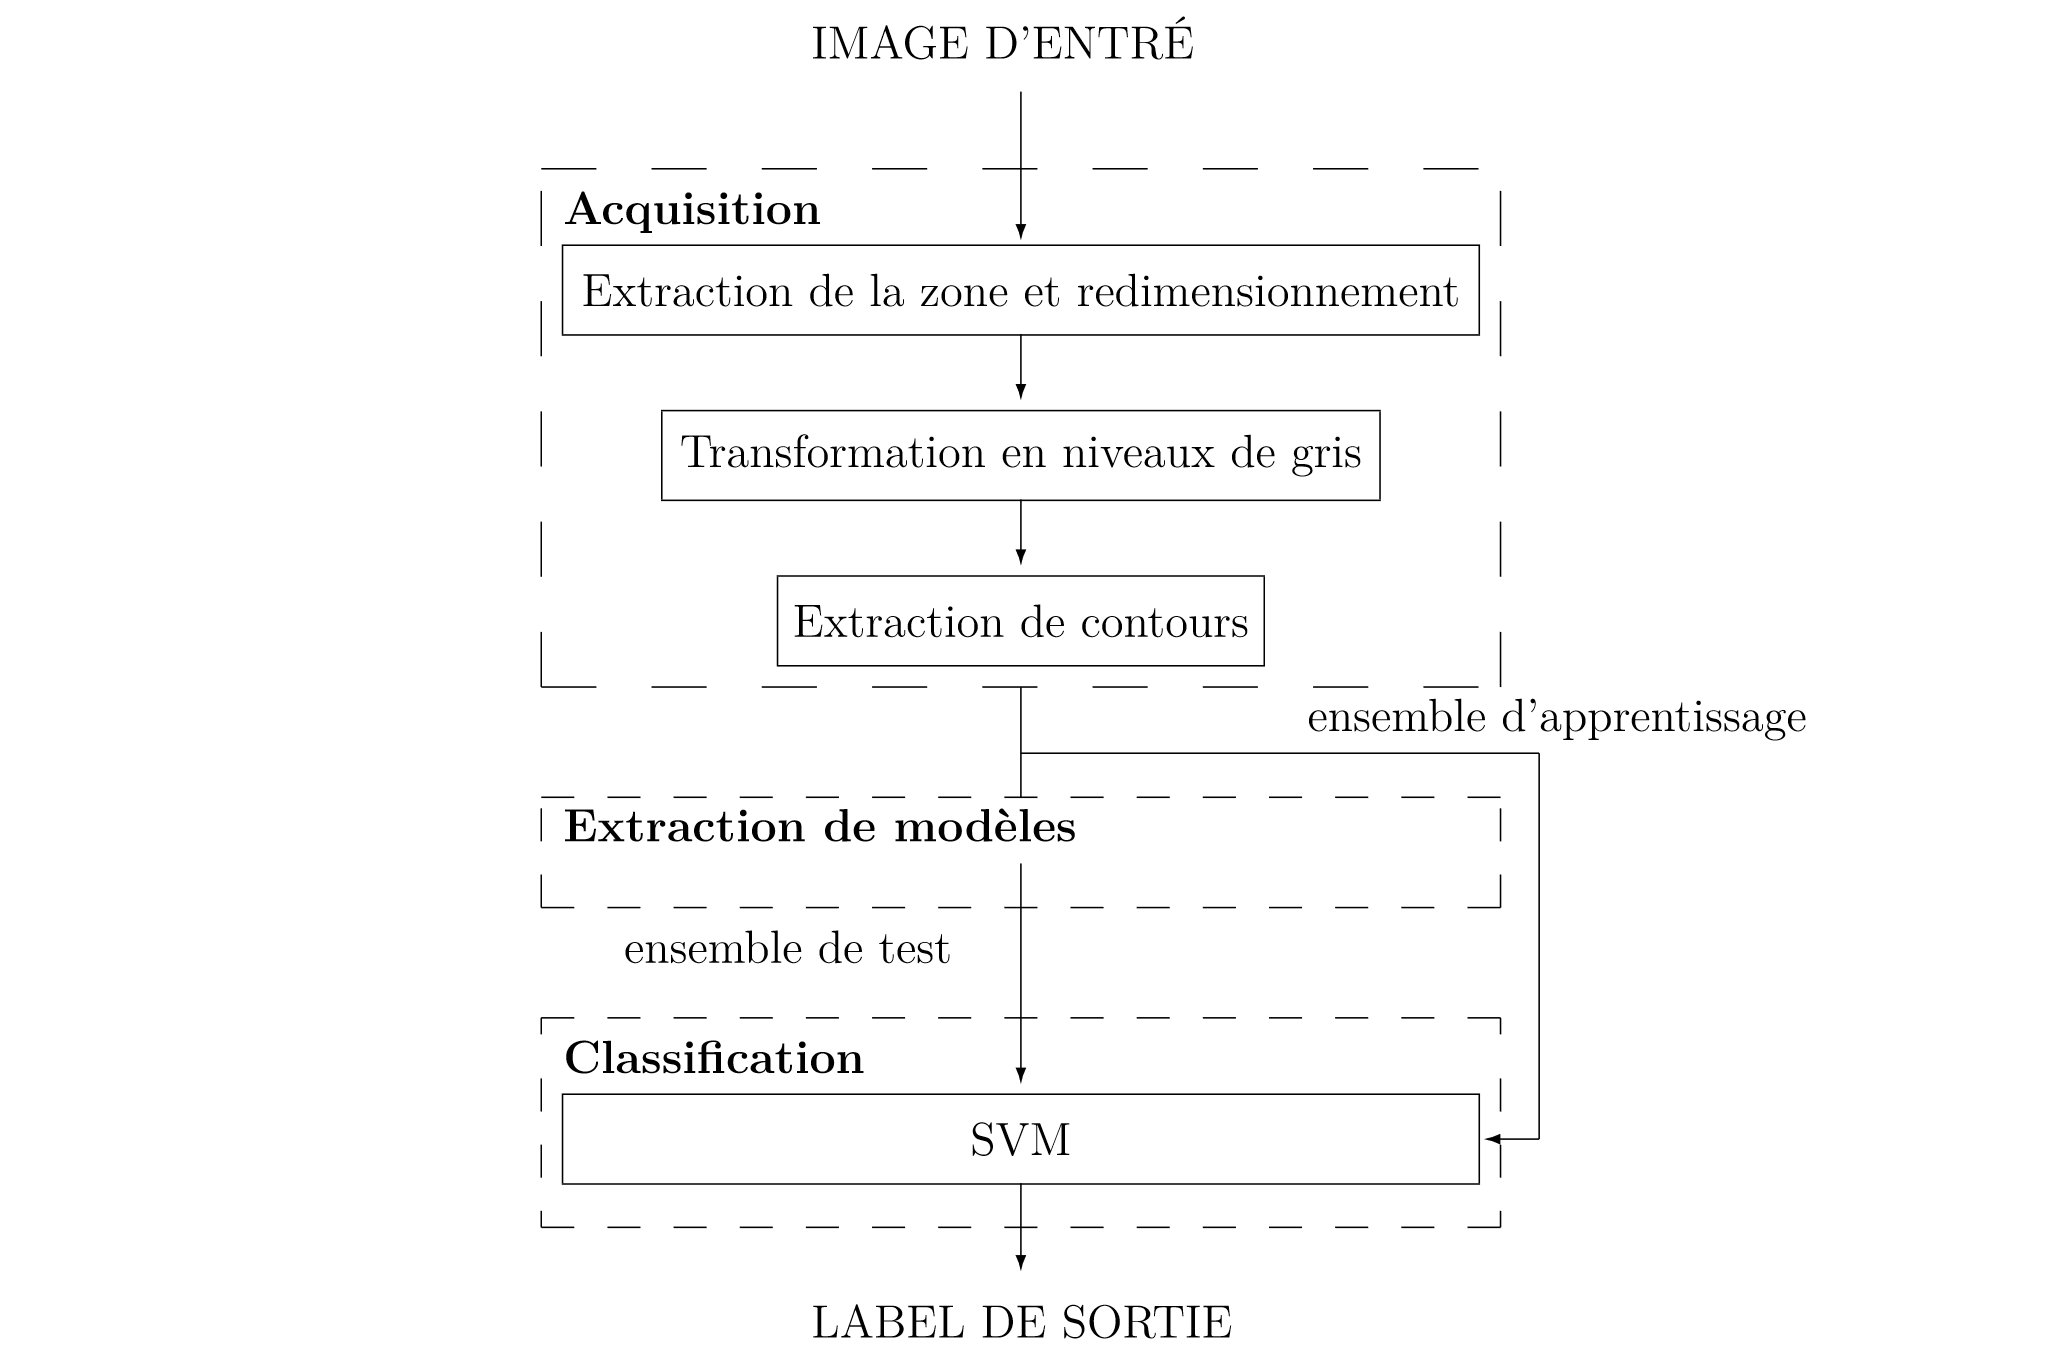
\includegraphics[scale=0.3]{data/svm.png}
\caption{Schéma de l'architecture pour le test de la difficulté du problème de test de l'architecture du réseau de neurones impulsionnels}
\label{svm}
\end{figure}
%\begin{picture}(16.8, 15)
	% Preprocess
    %\put(4.05, 7.4){\dashbox{0.5}(8.7,4.7)}
    %\put(4.25, 11.6){\shortstack{\textbf{Acquisition}}}
    %\put(4.25, 10.6){\framebox(8.3, 0.8)[c]{Extraction de la zone et redimensionnement}}
    %\put(5.15, 9.1){\framebox(6.5, 0.8)[c]{Transformation en niveaux de gris}}
	%\put(6.2, 7.6){\framebox(4.4, 0.8)[c]{Extraction de contours}}
    
    % feature extraction
    %\put(4.05, 5.4){\dashbox{0.3}(8.7, 1)}
    %\put(4.25, 6){\shortstack{\textbf{Extraction de modèles}}}
    
    % classification
    %\put(4.05, 2.5){\dashbox{0.3}(8.7, 1.9)}
    %\put(4.25, 3.9){\shortstack{\textbf{Classification}}}
    %\put(4.25, 2.9){\framebox(8.3, 0.8)[c]{SVM}}

	% labels
	%\put(4.8, 4.9){\shortstack{ensemble de test}}
    %\put(11, 7){\shortstack{ensemble d'apprentissage}}
    %\put(6.9, 4.7){\shortstack{vecteur de poids}}
    %\put(10, 1.4){\shortstack{Spikes d'apprentissage}}
    %\put(6.5, 13.1){\shortstack{IMAGE D’ENTRÉ}}
	%\put(6.5, 1.5){\shortstack{LABEL DE SORTIE}}

	% Les flèches entre les boîtes
    %\put(8.4, 2.9){\vector(0, -1){0.8}}
    %\put(8.4, 5.8){\vector(0, -1){2}}
    %\put(8.4, 12.8){\vector(0, -1){1.35}}
	%\put(8.4, 10.6){\vector(0, -1){0.6}}
    %\put(8.4, 9.1){\vector(0, -1){0.6}}
    %\put(8.4, 7.4){\line(0, -1){1}}
    %\put(8.4, 6.8){\line(1, 0){4.7}}
    	%\put(13.1, 6.8){\line(0, -1){3.5}} \put(13.1, 3.3){\vector(-1,0){0.5}}
	    %\put(8.4, 6.8){\line(-1, 0){4.4}} \put(4, 6.8){\vector(0, -1){0.8}}
    	%\put(8.4, 6.8){\line(1, 0){4.4}} \put(12.8, 6.8){\vector(0, -1){1.5}}
     %\put(10, 4.6){\vector(-1, 0){3}}
     %\put(12.8, 3.9){\line(0, -1){2.1}} \put(12.8, 1.8){\vector(-1, 0){4.6}}
%\end{picture}


\thispagestyle{empty}
\pagebreak

\section*{ANNEXE B :}
\begin{figure}[h!]
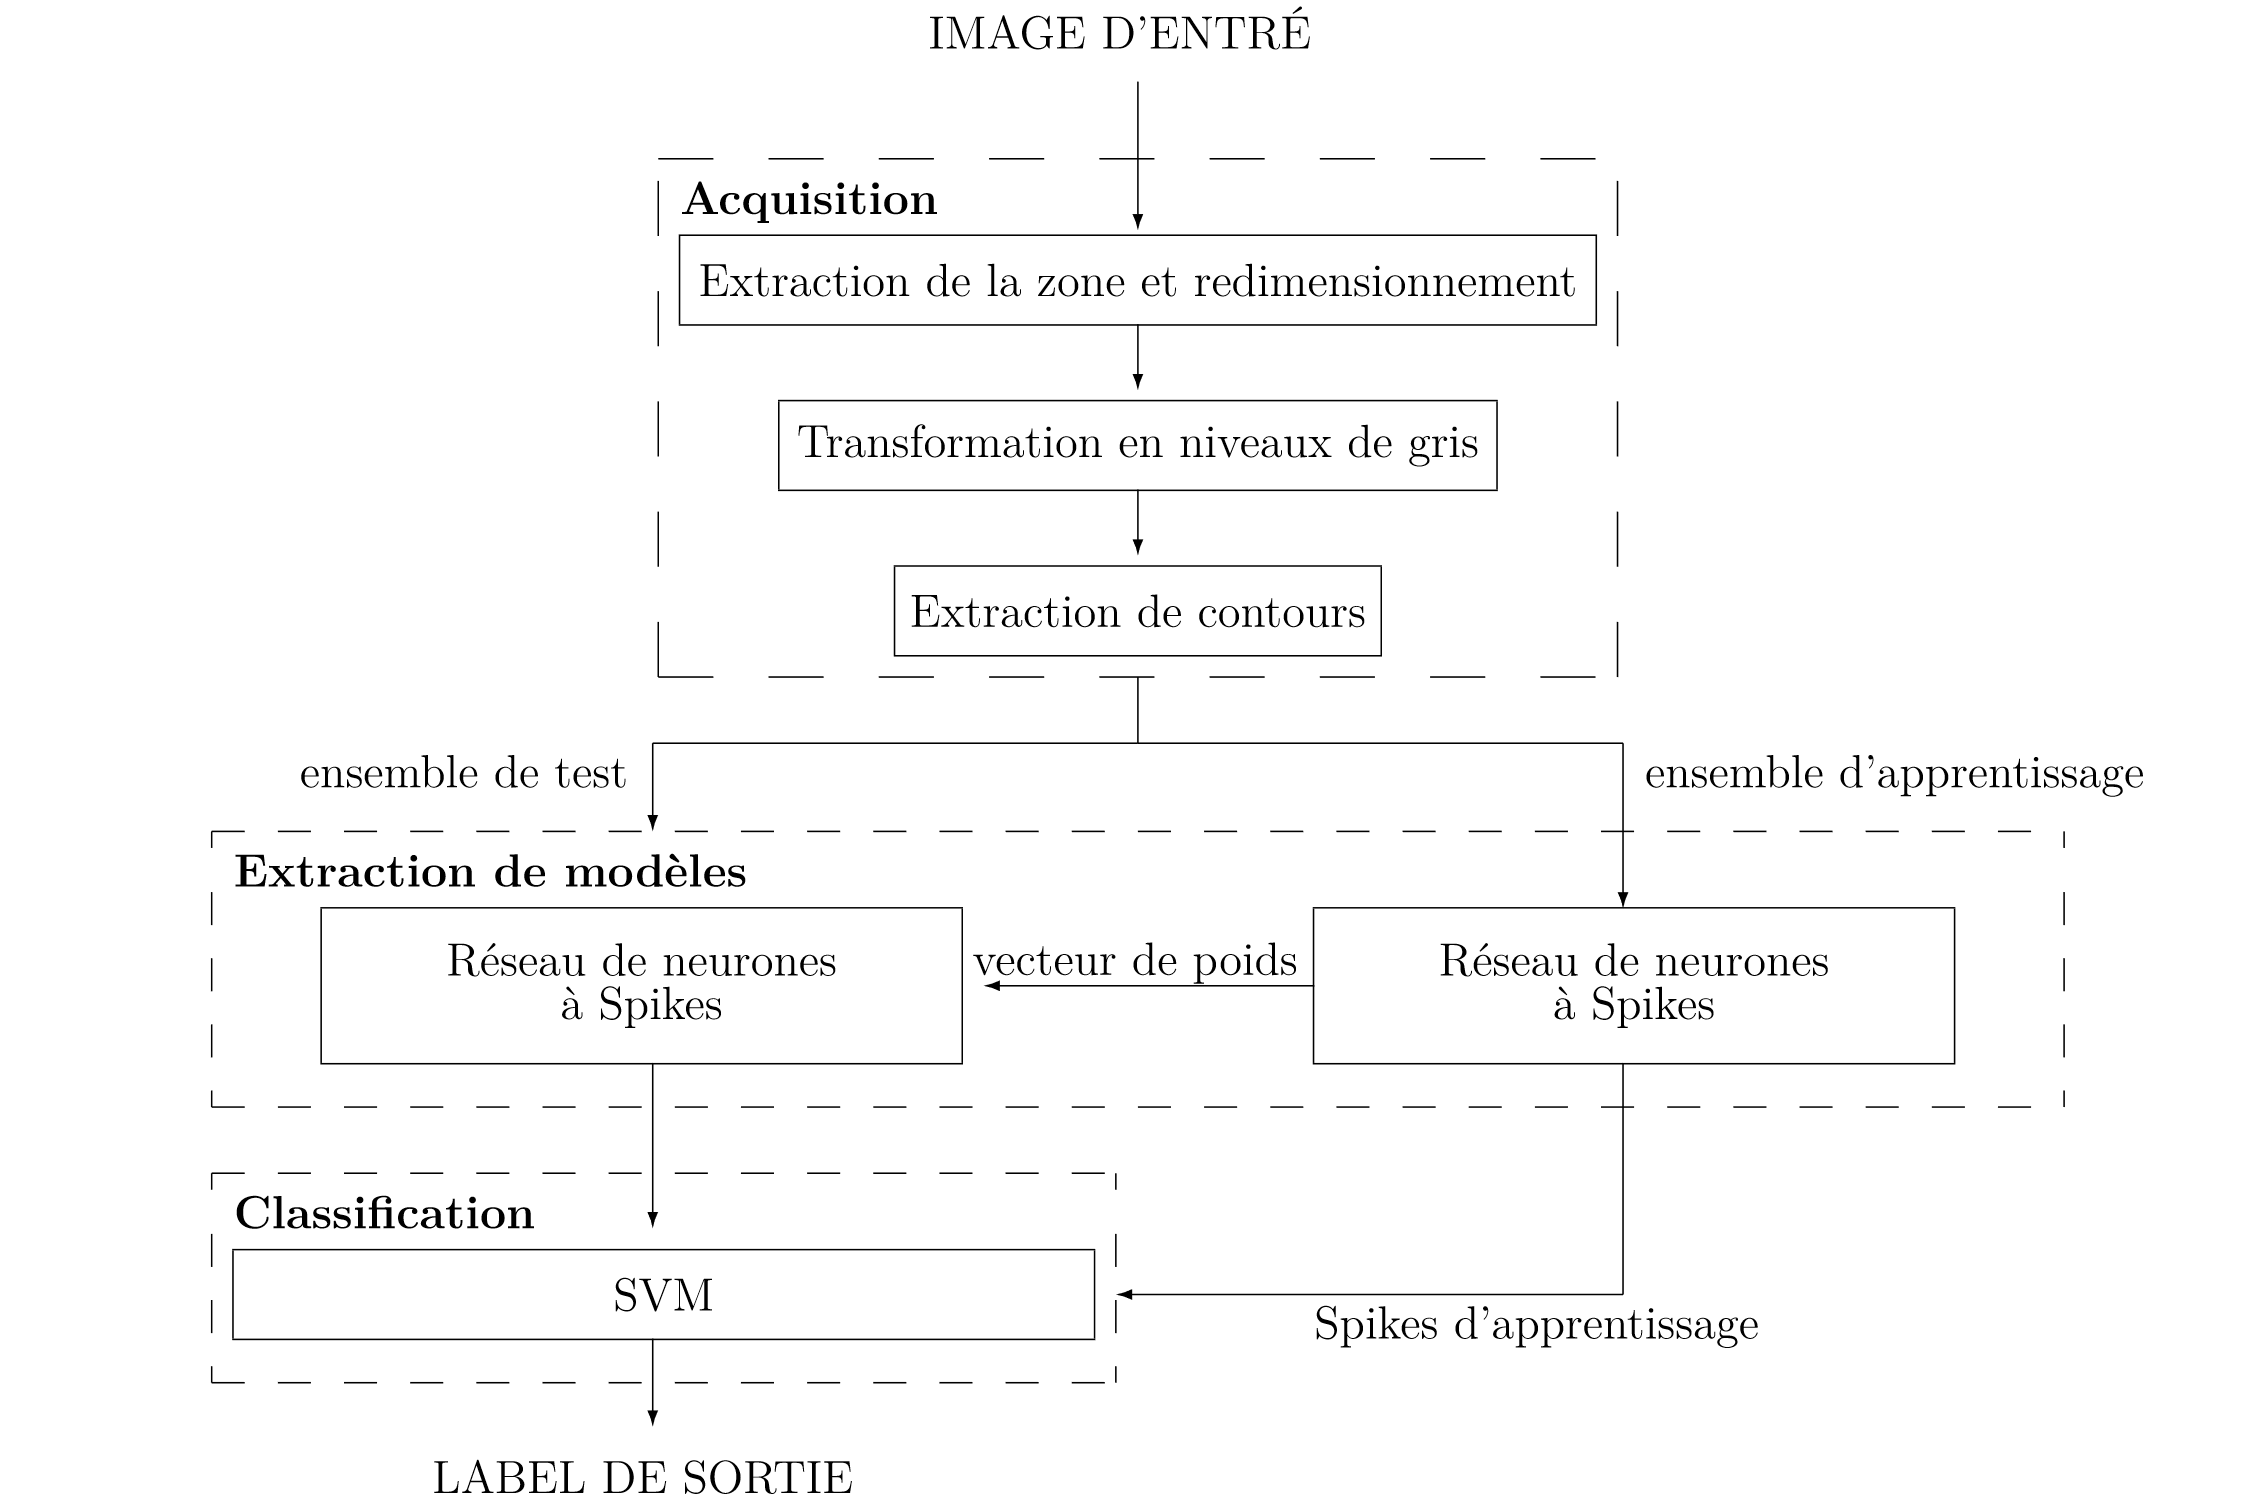
\includegraphics[scale=0.3]{data/archi.png}
\caption{Schéma de l'architecture utilisé dans ce projet}
\label{archi}
\end{figure}

\thispagestyle{empty}
\pagebreak

%%%%%%%%%%%%%%
%%  BIBLIO  %%
%%%%%%%%%%%%%%
%\listoffigures

%\pagebreak
%\printnomenclature

%\pagebreak

\bibliographystyle{plain}
\bibliography{biblist}
\thispagestyle{empty}

\end{document}


%%%%%%%%%%%%%%%%%%%%%%%%%%%
%%  END OF THE DOCUMENT  %%
%%%%%%%%%%%%%%%%%%%%%%%%%%%
